\section{Konvekse mængder}
%
I forbindelse med mængder af vektorer er det vigtigt at definere \textbf{konvekse mængder}.
\begin{defn}{}{konveks}
En mængde $S \subset \R^n$ er \textbf{konveks}, hvis $\lambda \textbf{x} + (1- \lambda ) \textbf{y} \in S$ for ethvert $\textbf{x}, \textbf{y} \in S$ og ethvert $\lambda \in [0,1]$. 
\end{defn}
\noindent
%
En mængde er med andre ord konveks, hvis ethvert element på en ret linje mellem to vilkårlige punkter $x$ og $y$ i mængden også tilhører mængden. 
På figur !REF HER! ses eksempler på konvekse og ikke-konvekse mængder. 
%
\begin{figure}[h!]
  \centering
  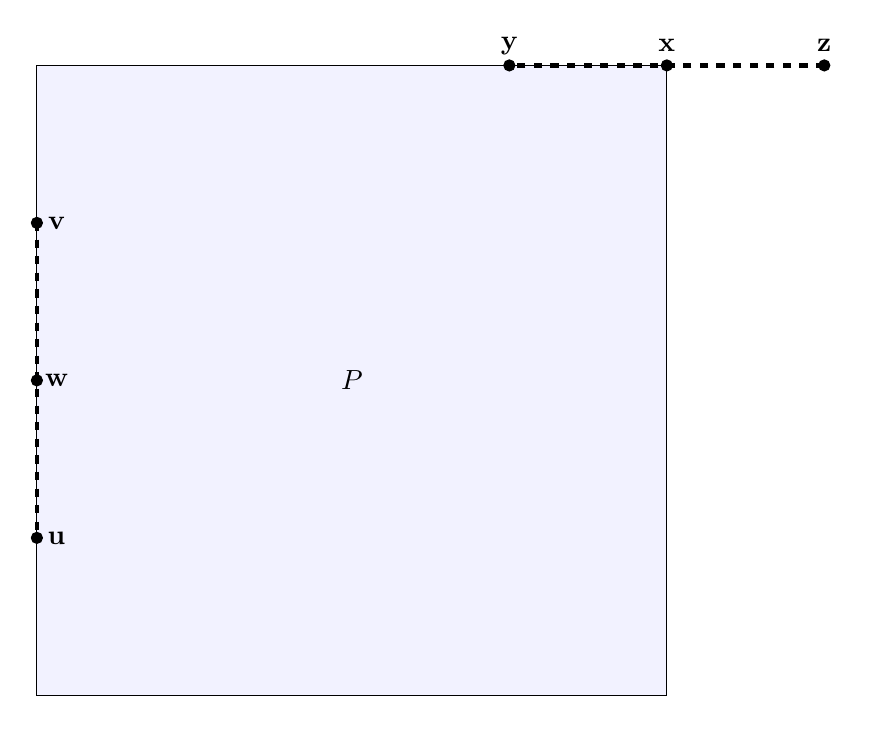
\begin{tikzpicture}
    \tikzset{punkt/.style={point, draw=black}} 
%   
% Punkter
% -------------------------------------------------
	\node at (4,4)	(1){};
	\node at (-4,4)	(4){};
	\node at (4,-4)	(2){};
	\node at (-4,-4) (3){};
	\node at (-4,-4) (3){};
	\node at (-4,-4) (3){};
% 
% 
	\filldraw[black, fill=blue!5] (2) rectangle (4);
	\node at (0,0) (P){$P$};
	
	\filldraw [black] (2,4) circle (2pt);
	\filldraw [black] (4,4) circle (2pt);
	\filldraw [black] (6,4) circle (2pt);
	\filldraw [black] (-4,2) circle (2pt);
	\filldraw [black] (-4,0) circle (2pt);
	\filldraw [black] (-4,-2) circle (2pt);	
	\node at (2,4.25)	 (y){$\textbf{y}$};
	\node at (4,4.25)	 (x){$\textbf{x}$};
	\node at (6,4.25)	 (z){$\textbf{z}$};
	\node at (-3.75,2)  (v){$\textbf{v}$};
	\node at (-3.75,0)	 (w){$\textbf{w}$};
	\node at (-3.75,-2) (u){$\textbf{u}$};


	\draw[-, dashed,black,ultra thick] (6,4) -- (2,4);
	\draw[-, dashed,black,ultra thick] (-4,2) -- (-4,-2);
  \end{tikzpicture}
  \caption{}
  \label{fig:konveks}
\end{figure}
%
\begin{defn}{}{konvekskombiskrog}
Lad $\textbf{x}^1, \textbf{x}^2, \ldots, \textbf{x}^k \in \R^n$, og $\lambda_1, \lambda_2, \ldots, \lambda_k$ være ikke-negative skalarer, hvis sum er $1$. 
\begin{enumerate}[label=(\alph*)]
	\item Vektoren $$\sum_{i=1}^{k} \lambda_i \textbf{x}^i$$ kaldes en \textbf{konveks kombination} af vektorerne $\textbf{x}^1, \textbf{x}^2, \ldots, \textbf{x}^k$. 
	\item Det \textbf{konvekse skrog} af vektorerne $\textbf{x}^1, \textbf{x}^2, \ldots, \textbf{x}^k$ er mængden af alle konvekse kombinationer af disse vektorer. 
%Det hedder vel ikke konvekse skrog, hvad kalder vi det? HORIA HJÆLP JENS
\end{enumerate}
\end{defn}
%
%Evt. noget metatekst
%
\begin{thm}{}{konveks}
\begin{enumerate}[label=(\alph*)]
	\item Skæringspunktet for konvekse mængder er konvekst. 
	%Hedder det skæringspunktet?? Jeg hidkalder Horia. 
	\item Enhver polyhedron er en konveks mængde.
	\item En konveks kombination af et endeligt antal elementer fra en konveks mængde tilhører også den mængde. 
	\item Det konvekse skrog af et endeligt antal vektorer er en konveks mængde. 
\end{enumerate}
\end{thm}
%
%
\begin{proof}
\begin{enumerate}[label=(\alph*)]
	\item Lad $I$ være en indeksmængde, lad $S_i$, $i \in I$, være et antal konvekse mængder, samt lad $ \lambda \in [0,1]$.
Antag nu, at vektorerne $\textbf{x}$ og $\textbf{y}$ tilhører fællesmængden $ \bigcap_{i \in I} S_i$. Det haves, at $ \lambda \textbf{x} + (1 - \lambda )\textbf{y} \in S_i$, eftersom enhver $S_i$ er konveks. Derfor er $ \bigcap_{i \in I} S_i$ konveks, da $ \lambda \textbf{x} + (1 - \lambda )\textbf{y} \in  \bigcap_{i \in I} S_i$, hvilket beviser (a). 
	\item Lad $\textbf{a}$ være en vektor, lad $b$ være en skalar, samt lad $ \lambda \in [0,1]$. 
Antag, at $\textbf{x}$ og $\textbf{y}$ henholdsvis opfylder, at $\textbf{a}^T \textbf{x} \geq b$ og $\textbf{a}^T \textbf{y} \geq b$, således de tilhører samme halvrum. 
Så er $\textbf{a}^T (\lambda \textbf{x} + (1 - \lambda) \textbf{y} ) \geq \lambda b + (1 - \lambda ) b = b$, hvilket beviser, at $ \lambda \textbf{x} + (1 - \lambda )\textbf{y}$ tilhører samme halvrum, hvormed halvrummet er konvekst.
Bemærk, at en polyhedron er fællesmængden af et endeligt antal halvrum, og at (b) dermed er bevist jævnfør (a). 
	\item Hmmmm
	\item Lad $S$ være et konvekst skrog af $\textbf{x}_1, \textbf{x}_2, \ldots, \textbf{x}_k$, samt lad $\textbf{y} = \sum_{i=1}^{k} \zeta_i \textbf{x}^i$, $\textbf{z} = \sum_{i=1}^{k} \theta_i \textbf{x}^i$ være to elementer i $S$, hvor $ \zeta_i \geq 0$, $ \theta_i \geq 0$, og $ \sum_{i=1}^{k} \zeta_i = \sum_{i=1}^{k} \theta_i = 1$. 
	Lad $ \lambda = [0,1]$. Så er $$\lambda \textbf{y} + (1 - \lambda ) \textbf{z} = \lambda \sum_{i=1}^k \zeta_i \textbf{x}^i + (1 - \lambda) \sum_{i=1}^k \theta_i \textbf{x}^i = \sum_{i=1}^k (\lambda \zeta_i + (1-\lambda )\theta_i ) \textbf{x}^i.$$
Bemærk, at koefficienterne $ \lambda \zeta_i + (1 - \lambda) \theta_i$, $i = 1, \ldots, k$, summerer til $1$ og ikke er negative. Dermed er $ \lambda \textbf{y} + (1 - \lambda ) \textbf{z}$ en konveks kombination af vektorerne $\textbf{x}^1, \ldots, \textbf{x}^k$, og tilhører derfor mængden $S$, hvormed (d) er bevist. 
\end{enumerate}
\end{proof}